\chapter{Defining colorings}

\section{The general concept of coloring}

As we will be working with many types of colorings, we introduce a general notion of an abstract coloring, which all specific types will share, in order to avoid repetition.

\begin{defn}[partial function]
    A \emph{partial function} is a function $f : X \rightarrow Y$ such that for all $x \in X$, either $f(x) \in Y$ or $f(x)$ is undefined.
\end{defn}

Since we are concerned with graphs of Platonic and Archimedean solids, which are all planar, we define the concept of coloring directly on their plane graphs, i.e. as they are drawn in the plane, rather than considering their abstract representations.

\begin{defn}[coloring]
    Let $S$ be a set, and let $G = (V, E, F)$ be a plane graph. We define a \emph{coloring} of $G$ as a partial function $c : V \cup E \cup F \rightarrow S$ together with a coloring rule $R$ that restricts which elements of the graph may be assigned the same color, i.e. mapped to the same element of $S$.
\end{defn}

In other words, a coloring is an assignment of elements in $S$ to vertices, edges, or faces of some plane graph. We can think of elements of $S$ as colors, but usually we will use numbers instead. What is especially important to us is whether any two elements are mapped onto the same target, i.e. colored by the same color. The coloring rule then prevents some assignments from being considered valid. This makes the coloring problem non-trivial.

\begin{defn}[family of colorings]
    For a graph $G$, let the set of all the colorings of $G$ sharing the same coloring rule $R$ be called a \emph{family of colorings} of $G$.
\end{defn}

\begin{defn}[$k$-coloring]
    Let $G = (V, E, F)$ be a plane graph. Let $C$ be a family of colorings of $G$. Let $S$ be a set such that $|S| = k$ for some $k \in \mathbb{N}$. A function $c \in C$ such that $c : V \cup E \cup F \rightarrow S$ is called a \emph{$k$-coloring} of $G$.
\end{defn}

Note that a $k$-coloring does not necessarily use all of the $k$ available colors. Mathematically speaking, a $k$-coloring is not necessarily a surjective function.

\begin{defn}[$k$-colorable graph]
    For a plane graph $G$, a family of colorings $C$, and a natural number $k$, if there exists a $k$-coloring of $G$, then we say that $G$ is \emph{$k$-colorable}.
\end{defn}

A typical question we ask when considering colorings of a graph is: What is the smallest number of colors that we can use to color the graph without violating the coloring rule? This leads to the definition of the so-called \textit{chromatic number}.


\begin{defn}[chromatic number]
    For a plane graph $G$ and a family of colorings $C$, the \emph{chromatic number} $\chi^C(G)$ is the minimum $k \in \mathbb{N}$ such that $G$ is $k$-colorable.
\end{defn}

Once we know a graph is $k$-colorable, there is another interesting property of the graph we can examine. We can ask how many different colorings with $k$ colors exist for the given graph. A closely related concept to this question is the \emph{chromatic polynomial}. But first, we need to define when two colorings are considered different.

\begin{defn}[different colorings]
    Given a plane graph $G = (V, E, F)$, a family of colorings $C$, and $k$-colorings $c_1, c_2 \in C$, we say $c_1$ and $c_2$ are \emph{different} if there exists $x \in V \cup E \cup F$ such that $c_1(x) \neq c_2(x)$.
\end{defn}

The above definition states that if two colorings assign different colors to any element, then the colorings are considered different. Note that this does not take into account any symmetries of the graph.

\begin{defn}[chromatic polynomial]
    For a graph $G$ and a family of colorings $C$, the \emph{chromatic polynomial}, denoted by $P_C(G,x)$ is a function such that for all $k \in \mathbb{N}$, we have $P_C(G,k) = n$, where $n$ is the number of different $k$-colorings of $G$.
\end{defn}

\section{Particular types of colorings}

\subsection{Vertex coloring}

\begin{defn}[vertex coloring]
    Given a set $S$ a \emph{vertex coloring} of a plane graph $G = (V, E, F)$ is any coloring $c : V \rightarrow S$ belonging to family of colorings with the following coloring rule:
    \begin{equation}\label{eqn:vtx_rule}
        \forall u, v \in V, \quad \text{if } \{u, v\} \in E, \text{ then } c(u) \neq c(v). 
        \tag{$R_V$}
    \end{equation}
    We denote this family of colorings by $X$.
\end{defn}

In other words, a vertex coloring is an assignment of colors to each vertex such that no two adjacent vertices share the same color.

\begin{figure}[H]
    \centering
    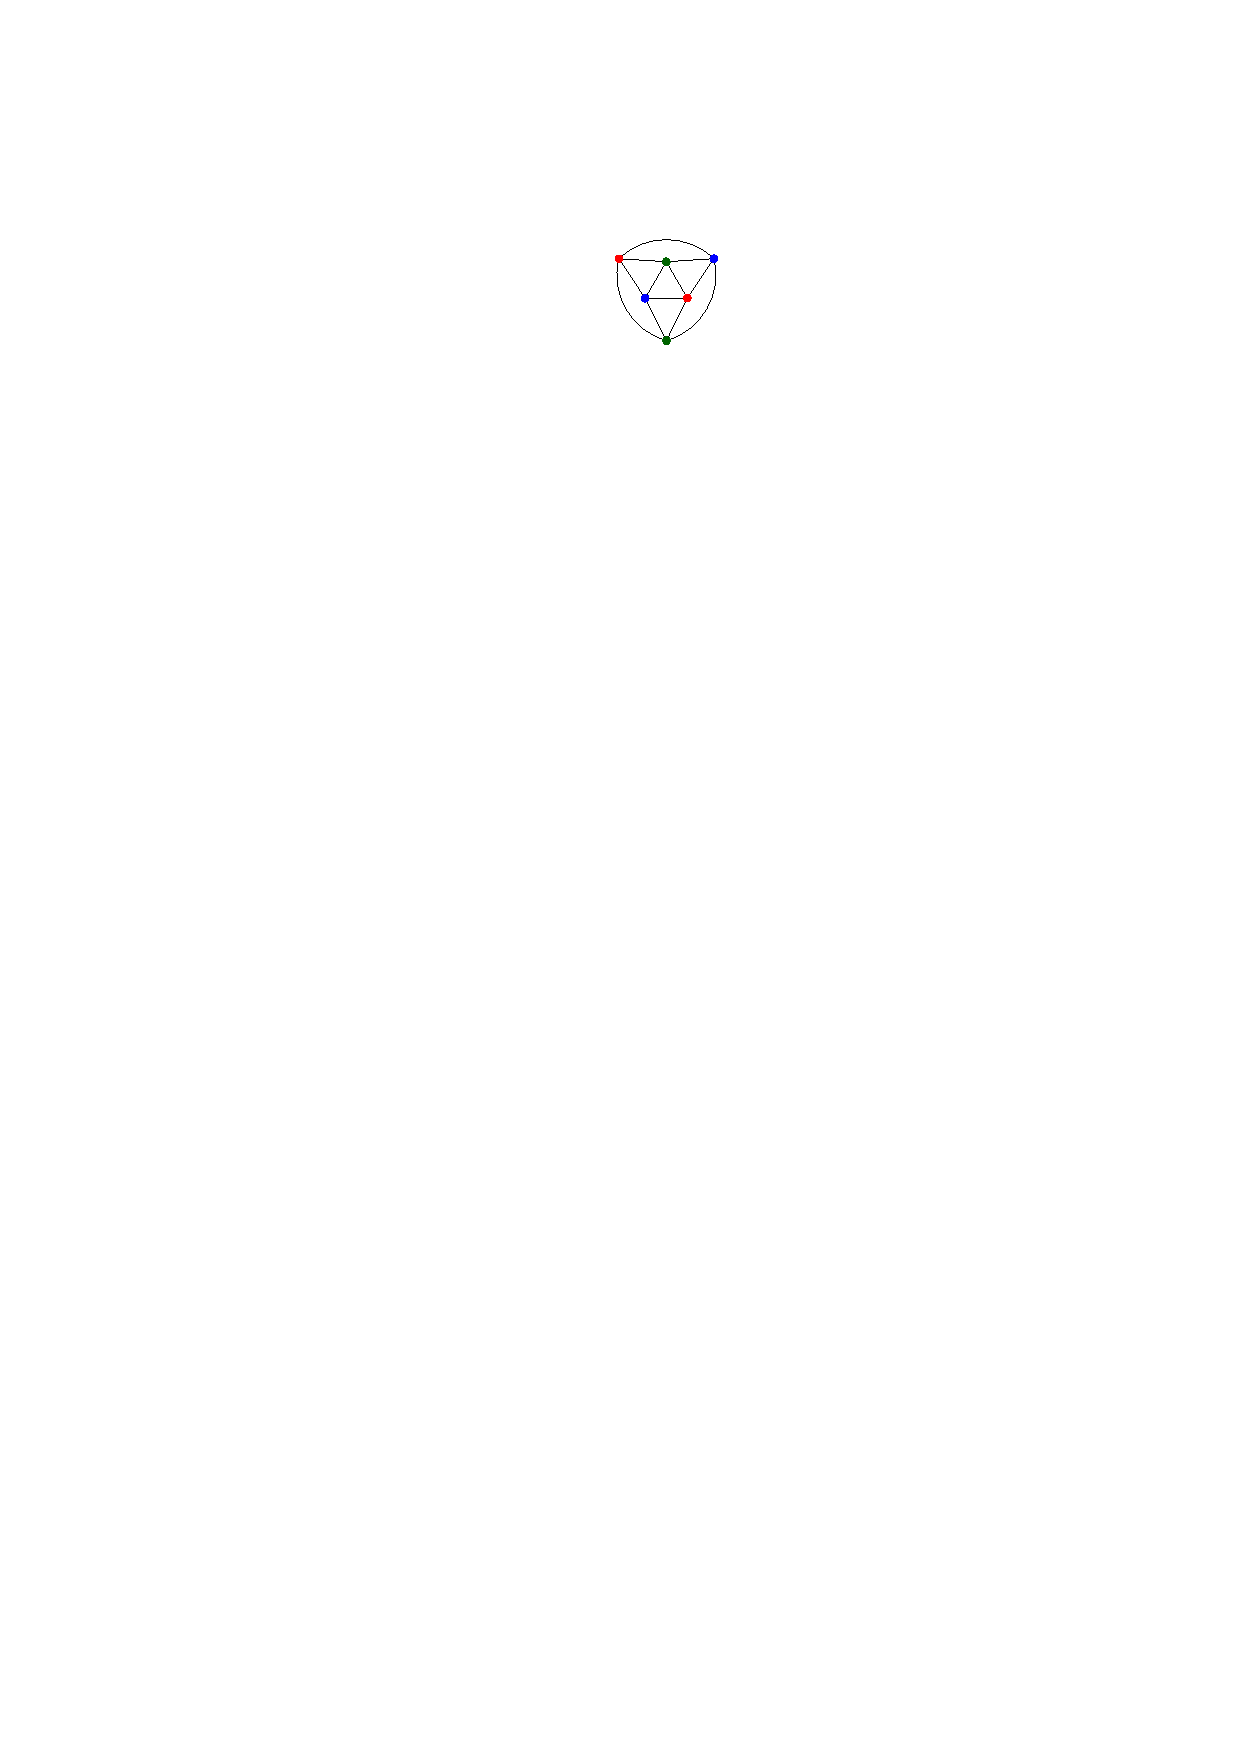
\includegraphics[width=0.20\textwidth]{../Resources/Figs/octahedral_vtx_colr.pdf}
    \caption{Vertex coloring of the octahedral graph}
    \label{fig:octahedral_vtx_coloring}
\end{figure}

The graph in Figure~\ref{fig:octahedral_vtx_coloring} has vertex chromatic number 3.

\subsection{Edge coloring}

\begin{defn}[edge coloring]
    Let $S$ be a set. An \emph{edge coloring} of a plane graph $G = (V, E, F)$ is a coloring $c : E \rightarrow S$ belonging to a family of colorings with the following rule: 
    \begin{equation}\label{eqn:edge_rule}
     \forall e, f \in E, \quad \text{ if } e \cap f \neq \emptyset, \text{ then } c(e) \neq c(f). \tag{$R_E$}
    \end{equation}
    We denote this family of colorings by $X'$.
   
\end{defn}

This rule states that any two edges sharing a common endpoint must be assigned different colors.

\begin{figure}[H]
    \centering
    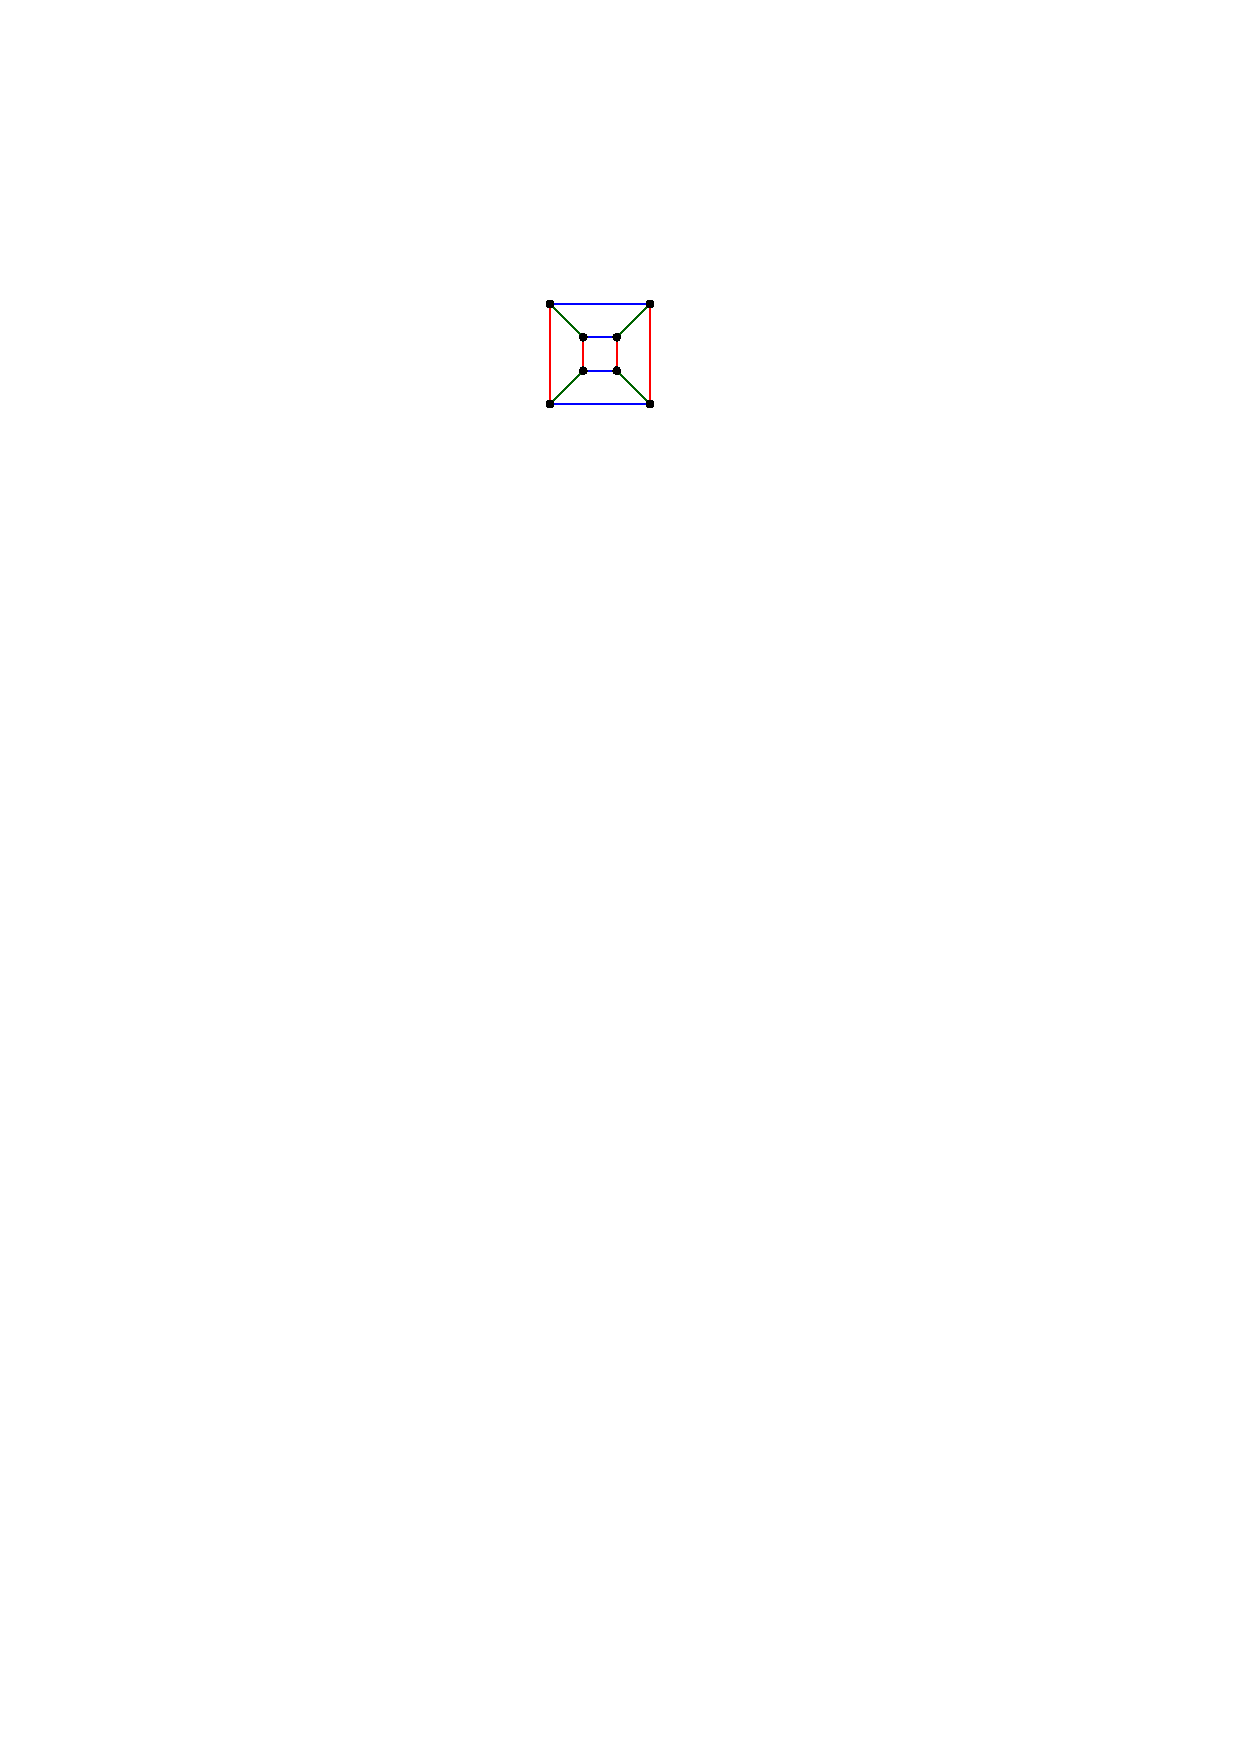
\includegraphics[width=0.2\textwidth]{../Resources/Figs/cubical_edg_colr.pdf}
    \caption{Edge coloring of the cubical graph}
    \label{fig:cubical_edge_coloring}
\end{figure}



\subsection{Total coloring}

By combining vertex and edge colorings and adding one additional constraint, we obtain the so-called \textit{total coloring} \cite{behzad65}.

\begin{defn}[total coloring]
    Given a set $S$ a \emph{total coloring} of a plane graph $G = (V, E, F)$ is a coloring $c : V \cup E \rightarrow S$ from a family of colorings sharing both coloring rules \ref{eqn:vtx_rule} and \ref{eqn:edge_rule}, as well as the following additional rule:
    \begin{equation}\label{eqn:tot_rule}
    \forall v \in V, \ \forall e \in E, \ \text{if } v \in e, \text{ then } c(v) \neq c(e). \tag{$R_T$}
    \end{equation}
    We denote this family of colorings by $X''$.
\end{defn}

\begin{figure}[H]
    \centering
    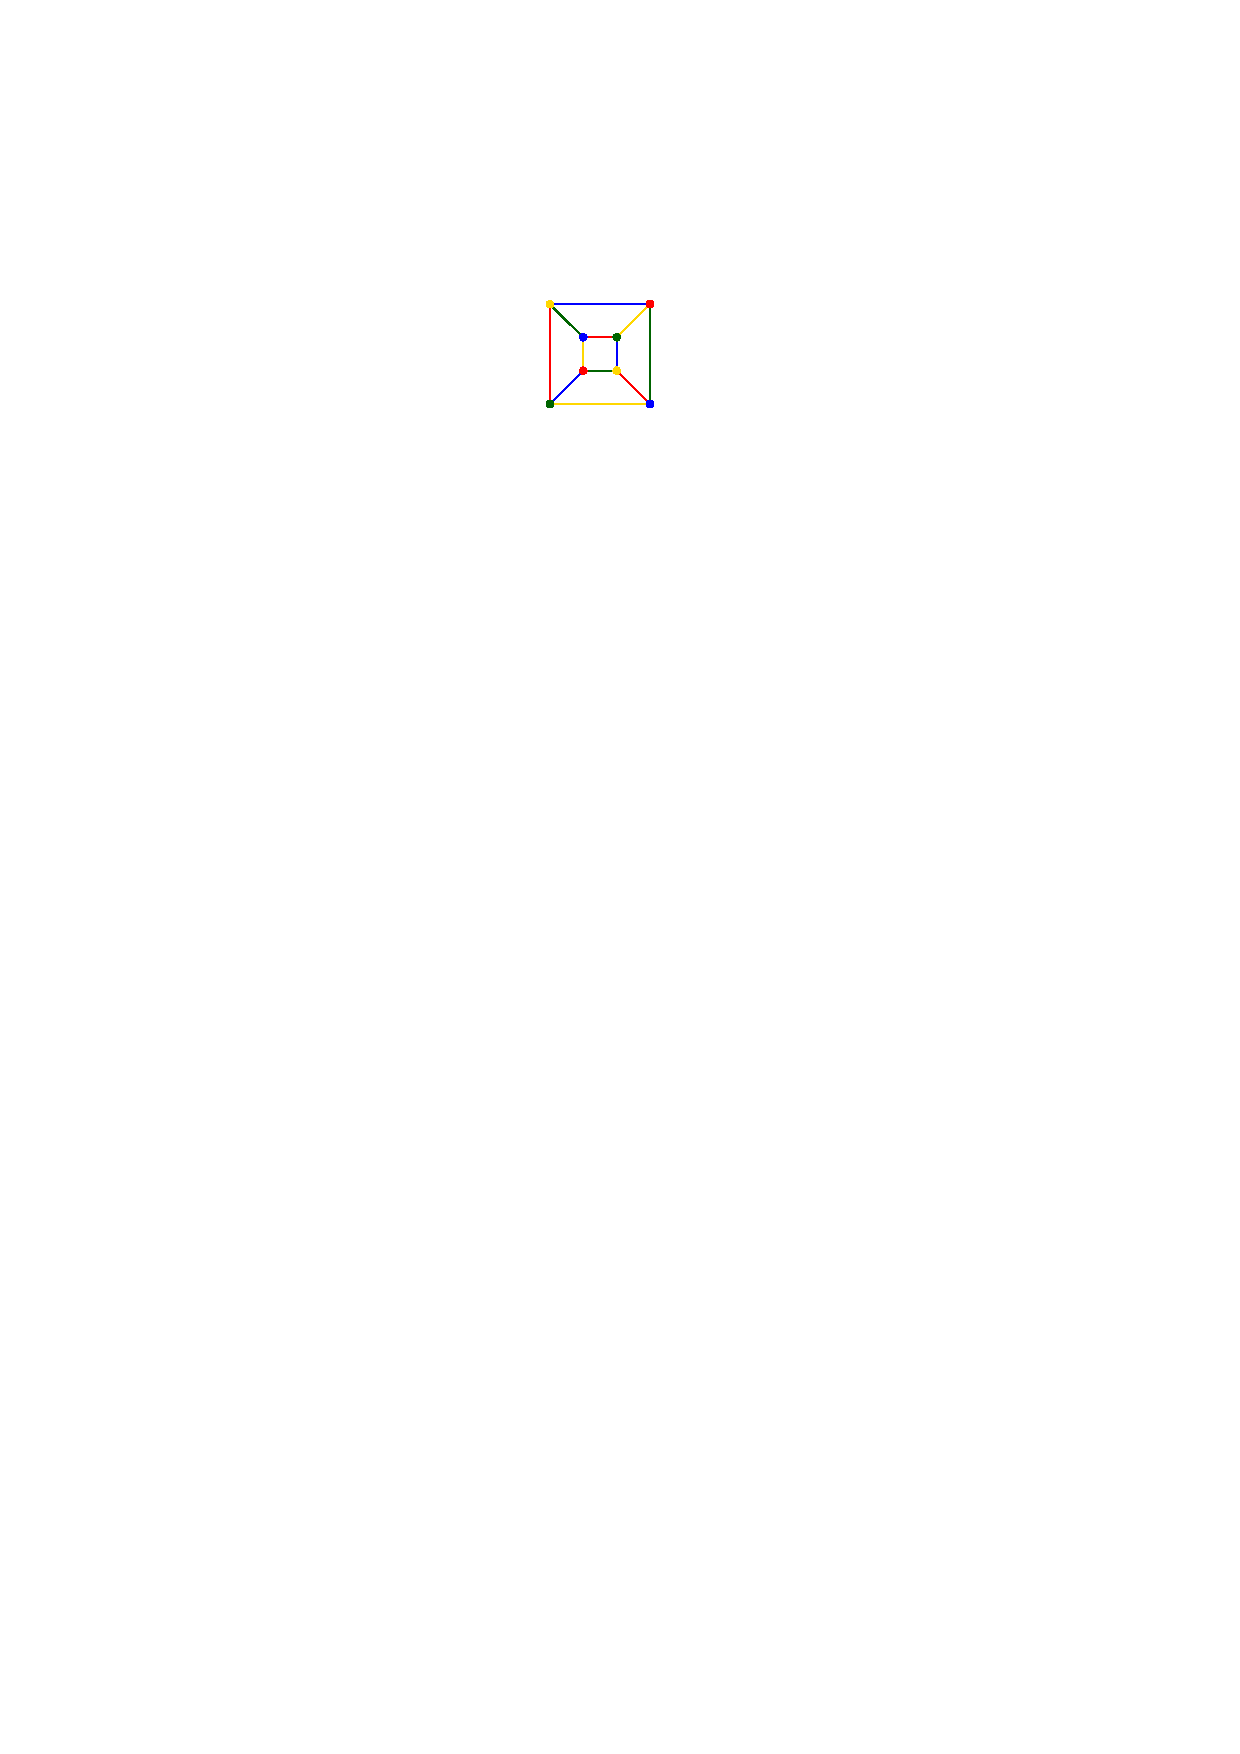
\includegraphics[width=0.2\textwidth]{../Resources/Figs/cubical_tot_colr_opt.pdf}
    \caption{Total coloring of the cubical graph using four colors}
    \label{fig:cubical_tot_coloring}
\end{figure}

\begin{figure}[H]
    \centering
    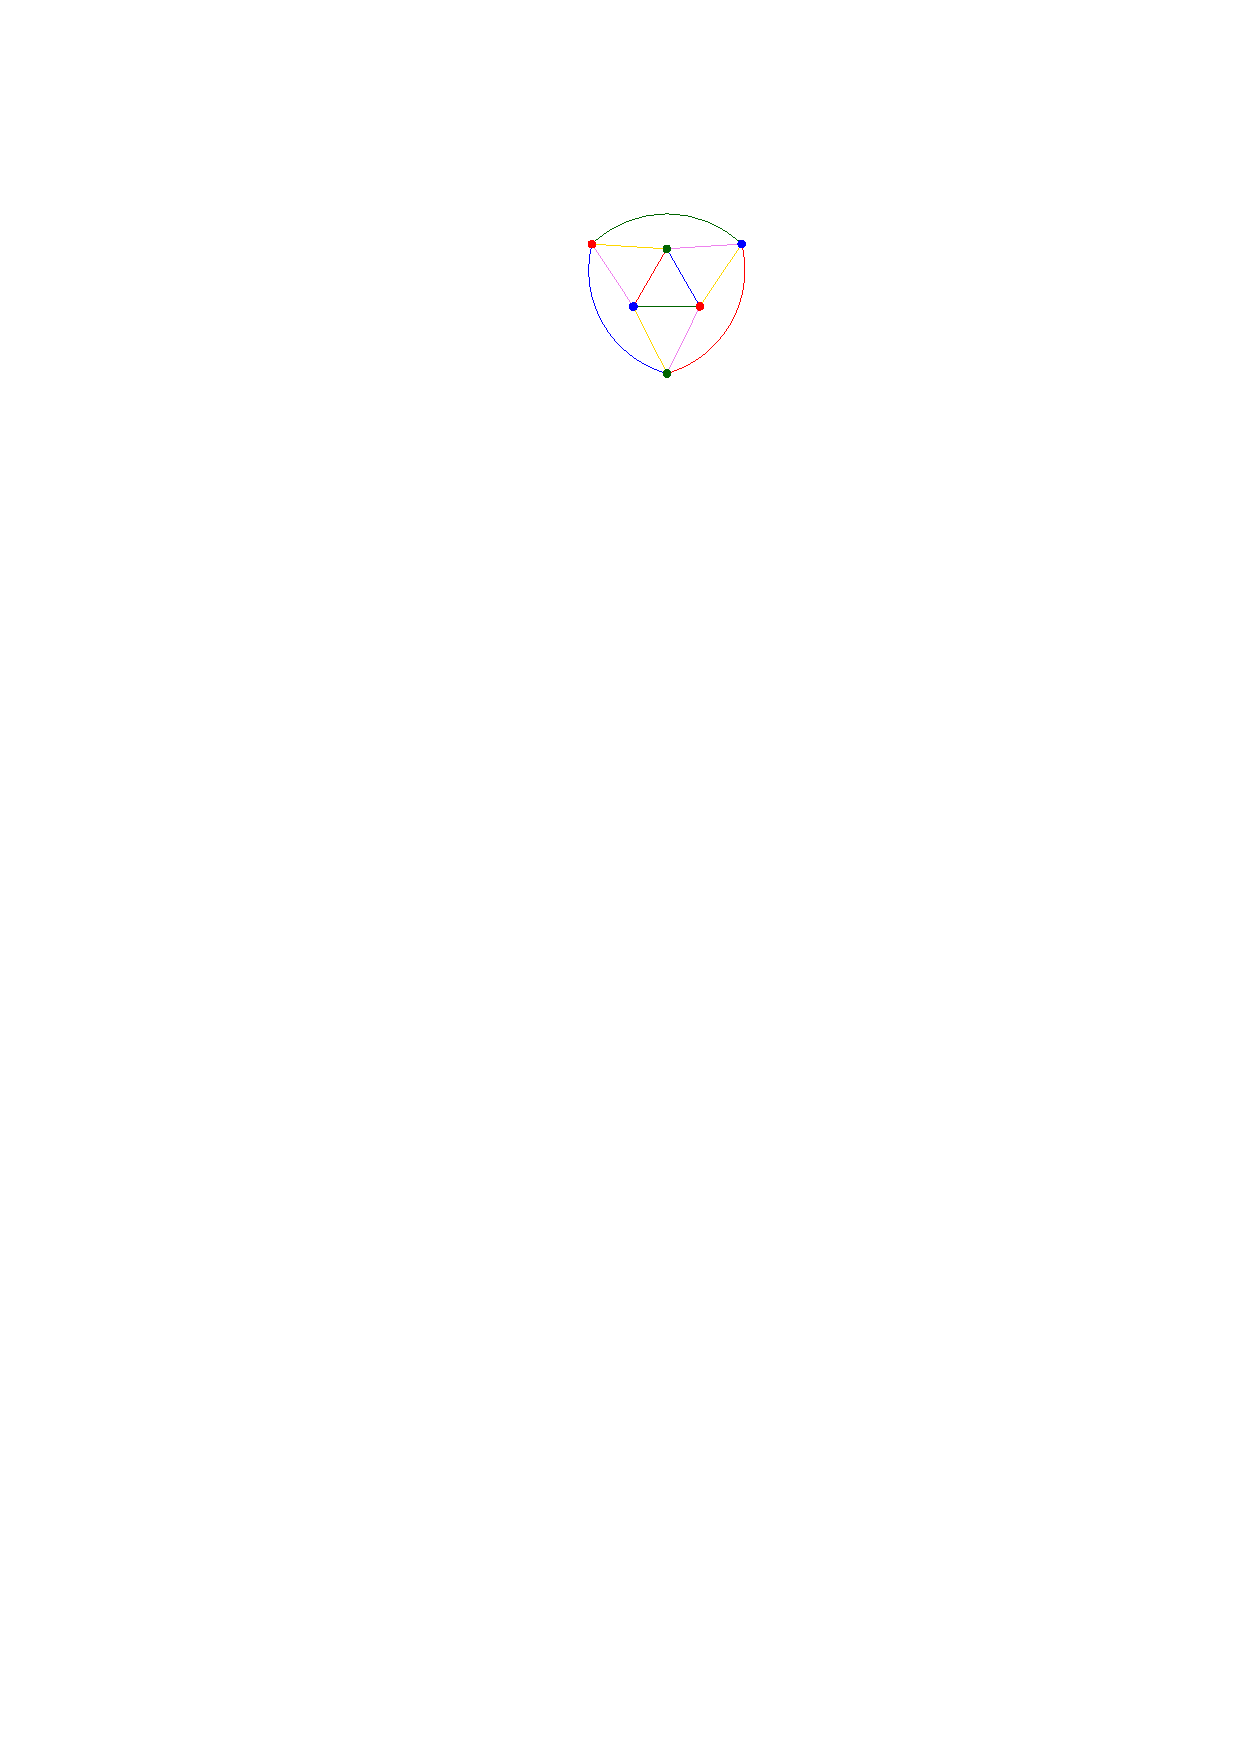
\includegraphics[width=0.25\textwidth]{../Resources/Figs/octahedral_tot_colr.pdf}
    \caption{Total coloring of the octahedral graph using five colors}
    \label{fig:octahedral_tot_coloring}
\end{figure}

\subsection{Face coloring}

Since we consider planar graphs, we can also color the faces of the corresponding plane graphs.

\begin{defn}[boundary]
    For a plane graph $G=(V,E,F)$ and a face $R \in F$, we define the \emph{boundary} of $R$, denoted by $\bnd(R)$, as the set of all edges incident with $R$.
\end{defn}

\begin{defn}[face coloring]
    Given a set $S$ and a plane graph $G = (V, E, F)$, a \emph{face coloring} is any function $c : F \rightarrow S$ belonging to a family of colorings with the following coloring rule:
    \begin{equation}\label{eqn:face_rule}
     \forall R_1, R_2 \in F, \ \text{if } \bnd(R_1) \cap \bnd(R_2) \neq \emptyset, \text{ then } c(R_1) \neq c(R_2). \tag{$R_F$}
    \end{equation}
    We denote this family of colorings by $X^F$.
\end{defn}

\begin{figure}[H]
    \centering
    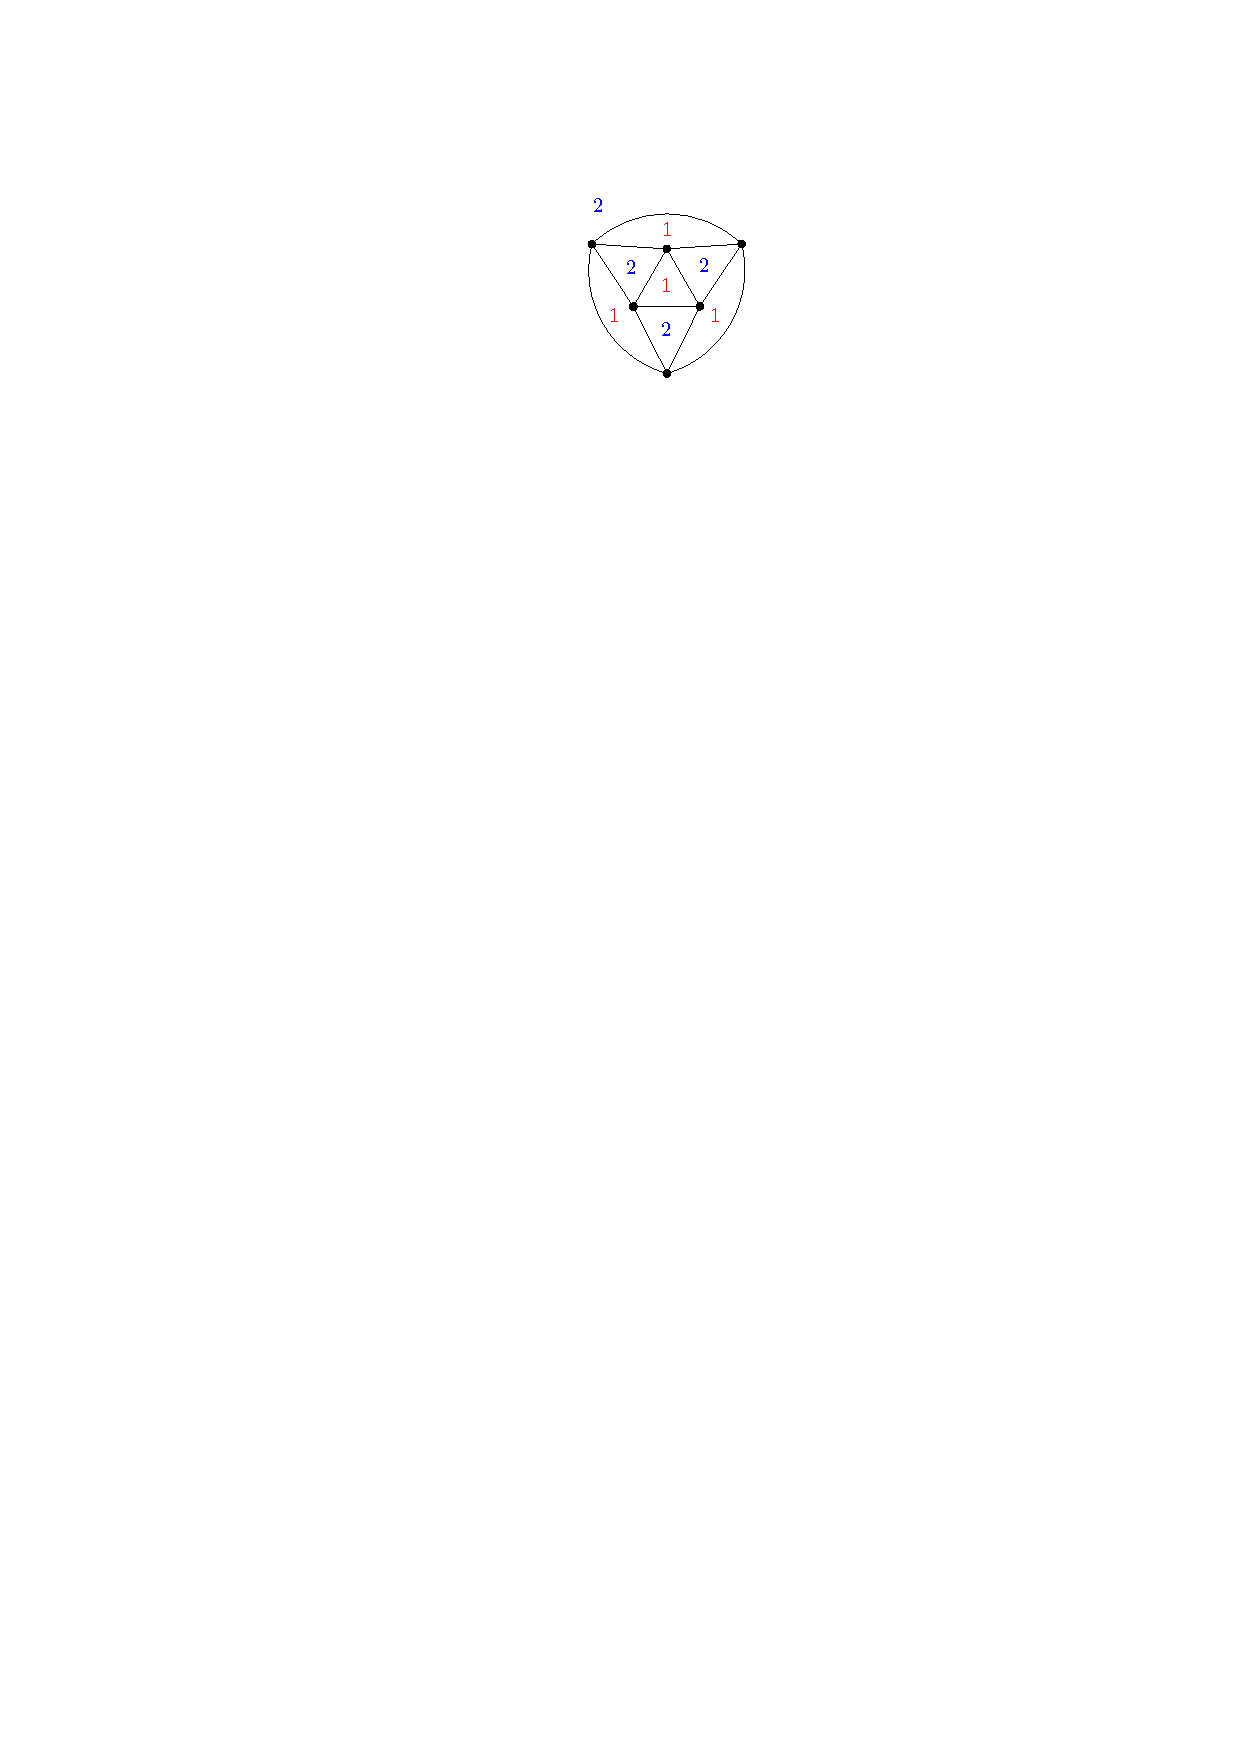
\includegraphics[width=0.2\textwidth]{../Resources/Figs/octahedral_face_colr.pdf}
    \caption{Face coloring of the octahedral graph using two colors (1 and 2)}
    \label{fig:face_tot_coloring}
\end{figure}

\subsection{Rainbow coloring}

So far, the particular colorings we have considered were all quite similar to each other. In what sense? All of their coloring rules were based on the notion of adjacency of some elements, i.e. neighboring vertices, incident edges etc. could not share the same color. There exist other types of colorings, where the coloring rules are based on other concepts, such as connectivity. One such example is the \textit{rainbow coloring} \cite{chartrand08}.

\begin{defn}[rainbow coloring]
    Let $S$ be a set. A \emph{rainbow coloring} of a plane graph $G = (V, E, F)$ is a coloring $c : E \rightarrow S$ belonging to a family of colorings with the following rule: 
    \begin{equation}\label{eqn:rainbow_rule}
     \forall u, v \in V, \ \exists uv \text{-path } (u, e_1, w_1, \ldots , w_{n-1}, e_n, v) \text{ s.t. } \forall i \neq j : c(e_i) \neq c(e_j). \tag{$R_R$}
    \end{equation}
    We denote this family of colorings by $X^R$.
\end{defn}

\begin{figure}[H]
    \centering
    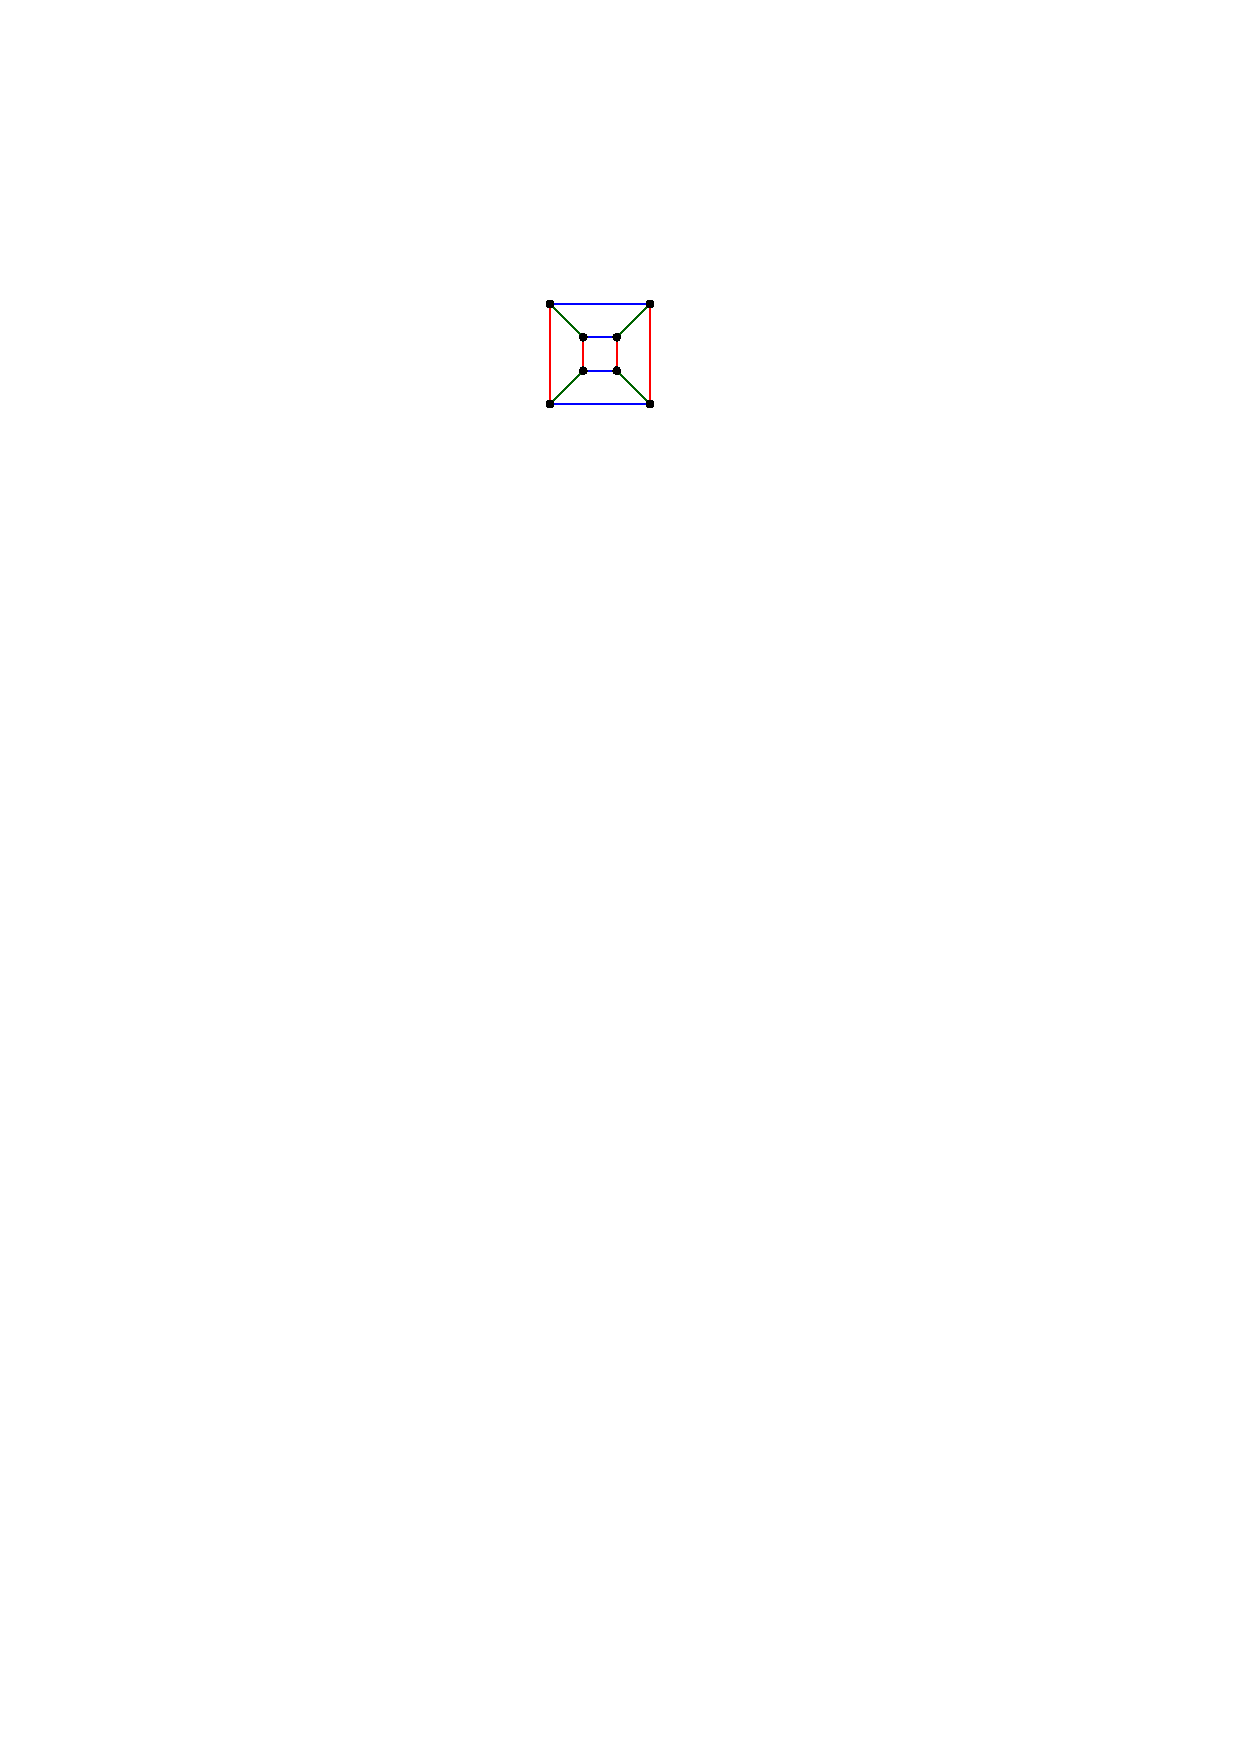
\includegraphics[width=0.2\textwidth]{../Resources/Figs/cubical_edg_colr.pdf}
    \caption{Rainbow coloring of the cubical graph. Let us appreciate the fact that it is also a proper edge coloring.}
    \label{fig:cubical_rainbow_coloring}
\end{figure}

\begin{figure}[H]
    \centering
    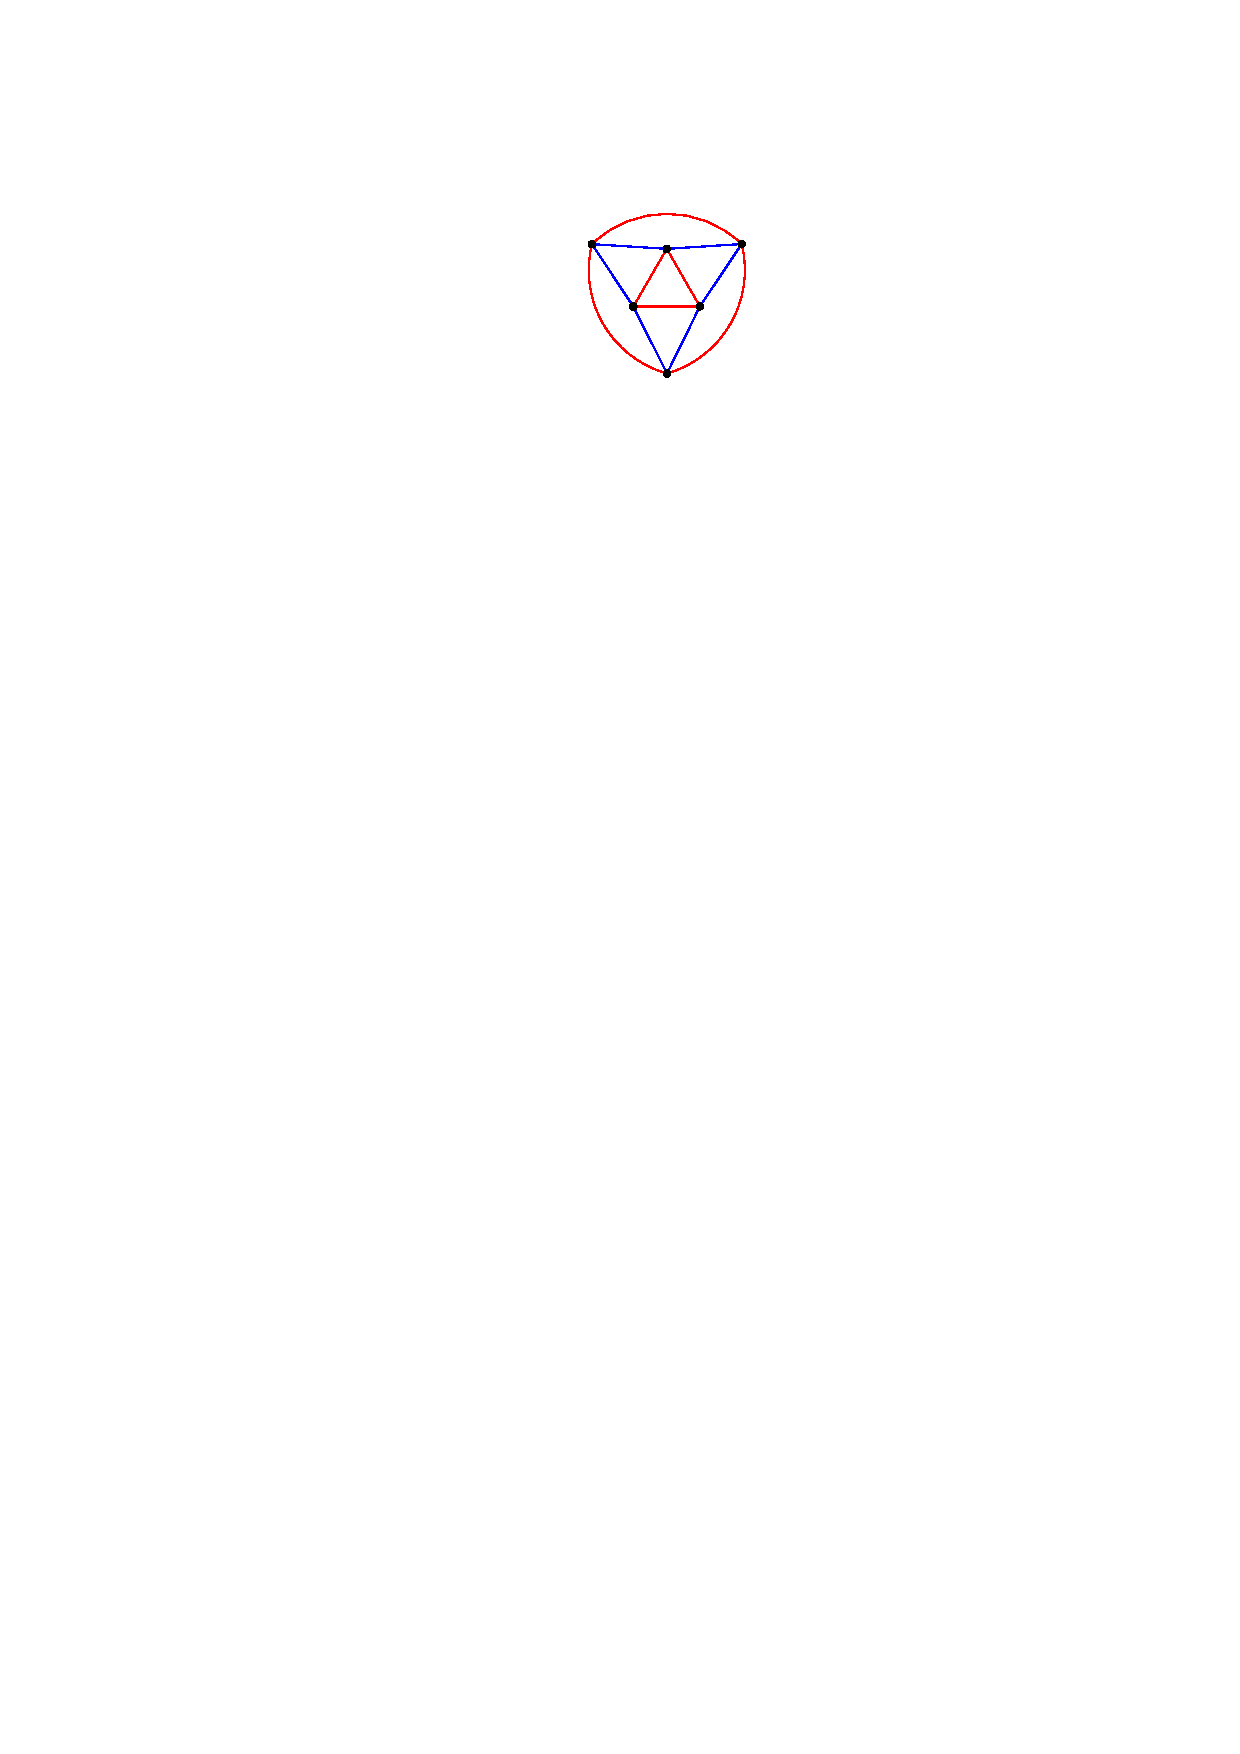
\includegraphics[width=0.25\textwidth]{../Resources/Figs/octahedral_rainbow_colr.pdf}
    \caption{Rainbow coloring of octahedral graph. Note that it is not a proper edge coloring.}
    \label{fig:octahedral_rainbow_coloring}
\end{figure}

\subsection{Magic labeling}

There also exist coloring rules that depend on the actual values of the colors. In such cases, the colors must come from a subset of the natural numbers, where arithmetic operations (such as addition) are defined. These colorings are usually referred to as \textit{labelings}.

All labelings share the notion of assigning a \textit{weight} to the elements of a graph. For an element $x$, we denote its weight by $w(x)$. Using this notation, we define an \textit{edge labeling} as a function $l : E \rightarrow \mathbb{N}$ and analogously, a \textit{vertex labeling} as a function $l : V \rightarrow \mathbb{N}$

Moreover, we call an edge labeling \textit{magic} if there exists $k \in \mathbb{N}$ such that $\forall v \in V: w(v) = k$, where $w$ is a weight function defined in terms of $l$. In other words, edge labeling $l$ is magic if all vertices have the same weight when edges are labeled using $l$. For example, we might define $w(v) = \sum_{uv \in E} l(uv)$. An analogous definition holds for magic vertex labeling.

All labeling definitions above are based on the book \textit{Magic Graphs} by Wallis \cite{marrwall2013}.